% Options for packages loaded elsewhere
\PassOptionsToPackage{unicode}{hyperref}
\PassOptionsToPackage{hyphens}{url}
%
\documentclass[
]{article}
\usepackage{amsmath,amssymb}
\usepackage{iftex}
\ifPDFTeX
  \usepackage[T1]{fontenc}
  \usepackage[utf8]{inputenc}
  \usepackage{textcomp} % provide euro and other symbols
\else % if luatex or xetex
  \usepackage{unicode-math} % this also loads fontspec
  \defaultfontfeatures{Scale=MatchLowercase}
  \defaultfontfeatures[\rmfamily]{Ligatures=TeX,Scale=1}
\fi
\usepackage{lmodern}
\ifPDFTeX\else
  % xetex/luatex font selection
\fi
% Use upquote if available, for straight quotes in verbatim environments
\IfFileExists{upquote.sty}{\usepackage{upquote}}{}
\IfFileExists{microtype.sty}{% use microtype if available
  \usepackage[]{microtype}
  \UseMicrotypeSet[protrusion]{basicmath} % disable protrusion for tt fonts
}{}
\makeatletter
\@ifundefined{KOMAClassName}{% if non-KOMA class
  \IfFileExists{parskip.sty}{%
    \usepackage{parskip}
  }{% else
    \setlength{\parindent}{0pt}
    \setlength{\parskip}{6pt plus 2pt minus 1pt}}
}{% if KOMA class
  \KOMAoptions{parskip=half}}
\makeatother
\usepackage{xcolor}
\usepackage[margin=1in]{geometry}
\usepackage{color}
\usepackage{fancyvrb}
\newcommand{\VerbBar}{|}
\newcommand{\VERB}{\Verb[commandchars=\\\{\}]}
\DefineVerbatimEnvironment{Highlighting}{Verbatim}{commandchars=\\\{\}}
% Add ',fontsize=\small' for more characters per line
\usepackage{framed}
\definecolor{shadecolor}{RGB}{248,248,248}
\newenvironment{Shaded}{\begin{snugshade}}{\end{snugshade}}
\newcommand{\AlertTok}[1]{\textcolor[rgb]{0.94,0.16,0.16}{#1}}
\newcommand{\AnnotationTok}[1]{\textcolor[rgb]{0.56,0.35,0.01}{\textbf{\textit{#1}}}}
\newcommand{\AttributeTok}[1]{\textcolor[rgb]{0.13,0.29,0.53}{#1}}
\newcommand{\BaseNTok}[1]{\textcolor[rgb]{0.00,0.00,0.81}{#1}}
\newcommand{\BuiltInTok}[1]{#1}
\newcommand{\CharTok}[1]{\textcolor[rgb]{0.31,0.60,0.02}{#1}}
\newcommand{\CommentTok}[1]{\textcolor[rgb]{0.56,0.35,0.01}{\textit{#1}}}
\newcommand{\CommentVarTok}[1]{\textcolor[rgb]{0.56,0.35,0.01}{\textbf{\textit{#1}}}}
\newcommand{\ConstantTok}[1]{\textcolor[rgb]{0.56,0.35,0.01}{#1}}
\newcommand{\ControlFlowTok}[1]{\textcolor[rgb]{0.13,0.29,0.53}{\textbf{#1}}}
\newcommand{\DataTypeTok}[1]{\textcolor[rgb]{0.13,0.29,0.53}{#1}}
\newcommand{\DecValTok}[1]{\textcolor[rgb]{0.00,0.00,0.81}{#1}}
\newcommand{\DocumentationTok}[1]{\textcolor[rgb]{0.56,0.35,0.01}{\textbf{\textit{#1}}}}
\newcommand{\ErrorTok}[1]{\textcolor[rgb]{0.64,0.00,0.00}{\textbf{#1}}}
\newcommand{\ExtensionTok}[1]{#1}
\newcommand{\FloatTok}[1]{\textcolor[rgb]{0.00,0.00,0.81}{#1}}
\newcommand{\FunctionTok}[1]{\textcolor[rgb]{0.13,0.29,0.53}{\textbf{#1}}}
\newcommand{\ImportTok}[1]{#1}
\newcommand{\InformationTok}[1]{\textcolor[rgb]{0.56,0.35,0.01}{\textbf{\textit{#1}}}}
\newcommand{\KeywordTok}[1]{\textcolor[rgb]{0.13,0.29,0.53}{\textbf{#1}}}
\newcommand{\NormalTok}[1]{#1}
\newcommand{\OperatorTok}[1]{\textcolor[rgb]{0.81,0.36,0.00}{\textbf{#1}}}
\newcommand{\OtherTok}[1]{\textcolor[rgb]{0.56,0.35,0.01}{#1}}
\newcommand{\PreprocessorTok}[1]{\textcolor[rgb]{0.56,0.35,0.01}{\textit{#1}}}
\newcommand{\RegionMarkerTok}[1]{#1}
\newcommand{\SpecialCharTok}[1]{\textcolor[rgb]{0.81,0.36,0.00}{\textbf{#1}}}
\newcommand{\SpecialStringTok}[1]{\textcolor[rgb]{0.31,0.60,0.02}{#1}}
\newcommand{\StringTok}[1]{\textcolor[rgb]{0.31,0.60,0.02}{#1}}
\newcommand{\VariableTok}[1]{\textcolor[rgb]{0.00,0.00,0.00}{#1}}
\newcommand{\VerbatimStringTok}[1]{\textcolor[rgb]{0.31,0.60,0.02}{#1}}
\newcommand{\WarningTok}[1]{\textcolor[rgb]{0.56,0.35,0.01}{\textbf{\textit{#1}}}}
\usepackage{graphicx}
\makeatletter
\def\maxwidth{\ifdim\Gin@nat@width>\linewidth\linewidth\else\Gin@nat@width\fi}
\def\maxheight{\ifdim\Gin@nat@height>\textheight\textheight\else\Gin@nat@height\fi}
\makeatother
% Scale images if necessary, so that they will not overflow the page
% margins by default, and it is still possible to overwrite the defaults
% using explicit options in \includegraphics[width, height, ...]{}
\setkeys{Gin}{width=\maxwidth,height=\maxheight,keepaspectratio}
% Set default figure placement to htbp
\makeatletter
\def\fps@figure{htbp}
\makeatother
\setlength{\emergencystretch}{3em} % prevent overfull lines
\providecommand{\tightlist}{%
  \setlength{\itemsep}{0pt}\setlength{\parskip}{0pt}}
\setcounter{secnumdepth}{-\maxdimen} % remove section numbering
\usepackage{amsmath}
\usepackage{mathtools}
\usepackage{amsthm}
\usepackage{bm}
\usepackage{xcolor}
\usepackage{siunitx}
\ifLuaTeX
  \usepackage{selnolig}  % disable illegal ligatures
\fi
\IfFileExists{bookmark.sty}{\usepackage{bookmark}}{\usepackage{hyperref}}
\IfFileExists{xurl.sty}{\usepackage{xurl}}{} % add URL line breaks if available
\urlstyle{same}
\hypersetup{
  pdftitle={Time Series Analysis - STAT 478 - HW \#6},
  pdfauthor={Alex Towell (atowell@siue.edu)},
  hidelinks,
  pdfcreator={LaTeX via pandoc}}

\title{Time Series Analysis - STAT 478 - HW \#6}
\author{Alex Towell
(\href{mailto:atowell@siue.edu}{\nolinkurl{atowell@siue.edu}})}
\date{}

\begin{document}
\maketitle

\newcommand{\var}{\operatorname{Var}}
\newcommand{\expect}{\operatorname{E}}
\newcommand{\corr}{\operatorname{Corr}}
\newcommand{\cov}{\operatorname{Cov}}
\newcommand{\ssr}{\operatorname{SSR}}
\newcommand{\se}{\operatorname{SE}}
\newcommand{\mat}[1]{\bm{#1}}
\newcommand{\eval}[2]{\left. #1 \right\vert_{#2}}
\newcommand{\argmin}{\operatorname{arg\,min}}

\hypertarget{problem-1}{%
\section{Problem 1}\label{problem-1}}

A data set of 324 measurements of an industrial robot's positions are in
the robot object in the TSA package.

\begin{Shaded}
\begin{Highlighting}[]
\FunctionTok{library}\NormalTok{(TSA)}
\FunctionTok{data}\NormalTok{(robot)}
\FunctionTok{head}\NormalTok{(robot)}
\end{Highlighting}
\end{Shaded}

\begin{verbatim}
## [1]  0.0011  0.0011  0.0024  0.0000 -0.0018  0.0055
\end{verbatim}

\hypertarget{preliminary-analysis}{%
\subsection{Preliminary analysis}\label{preliminary-analysis}}

We denote the industrial robot's position time series as \(\{P_t\}\). A
quick plot:

\begin{Shaded}
\begin{Highlighting}[]
\FunctionTok{plot}\NormalTok{(robot,}\AttributeTok{xlab=}\StringTok{"time"}\NormalTok{,}\AttributeTok{ylab=}\StringTok{"position"}\NormalTok{)}
\end{Highlighting}
\end{Shaded}


\includegraphics{hw6_files/figure-latex/unnamed-chunk-2-1.pdf}

\hypertarget{part-a}{%
\subsection{Part (a)}\label{part-a}}

\fbox{\begin{minipage}{.8\textwidth}
Fit an $\operatorname{AR}(1)$ model for these data.
Give the equation of the estimated model.
\end{minipage}}

We suppose that \(\{P_t\} \sim \operatorname{AR}(1)\), defined as \[
   P_t = c + \phi P_{t-1} + e_t
\] where \(e_t\) are the residuals in the model. If the model is a good
fit, \(e_t\) approximates \(\operatorname{WN}(0,\sigma_e^2)\), zero-mean
white noise.

We fit the data to the \(\operatorname{AR}(1)\) model with:

\begin{Shaded}
\begin{Highlighting}[]
\NormalTok{robot.ar1 }\OtherTok{\textless{}{-}} \FunctionTok{arima}\NormalTok{(robot,}\AttributeTok{order=}\FunctionTok{c}\NormalTok{(}\DecValTok{1}\NormalTok{,}\DecValTok{0}\NormalTok{,}\DecValTok{0}\NormalTok{))}
\FunctionTok{print}\NormalTok{(robot.ar1)}
\end{Highlighting}
\end{Shaded}

\begin{verbatim}
## 
## Call:
## arima(x = robot, order = c(1, 0, 0))
## 
## Coefficients:
##          ar1  intercept
##       0.3074     0.0015
## s.e.  0.0528     0.0002
## 
## sigma^2 estimated as 6.482e-06:  log likelihood = 1475.54,  aic = -2947.08
\end{verbatim}

\begin{Shaded}
\begin{Highlighting}[]
\NormalTok{robot.ar1.phi }\OtherTok{\textless{}{-}} \FunctionTok{coef}\NormalTok{(robot.ar1)[}\DecValTok{1}\NormalTok{]}
\NormalTok{robot.ar1.c }\OtherTok{\textless{}{-}} \FunctionTok{coef}\NormalTok{(robot.ar1)[}\DecValTok{2}\NormalTok{]}
\NormalTok{robot.ar1.mu }\OtherTok{\textless{}{-}}\NormalTok{ robot.ar1.c }\SpecialCharTok{/}\NormalTok{ (}\DecValTok{1}\SpecialCharTok{{-}}\NormalTok{robot.ar1.phi}\SpecialCharTok{\^{}}\DecValTok{2}\NormalTok{)}

\CommentTok{\# robot.ar1.resid \textless{}{-} robot.ar1 {-} robot}
\CommentTok{\# plot(robot.ar1.resid)}
\CommentTok{\# robot.ar1.resid.mu \textless{}{-} mean(robot.ar1.resid)}
\CommentTok{\# print(robot.ar1.resid.mu)}
\CommentTok{\# robot.ar1.resid.var \textless{}{-} var(robot.ar1.resid)}
\CommentTok{\# print(robot.ar1.resid.var)}
\end{Highlighting}
\end{Shaded}

The estimate of the \(\operatorname{AR}(1)\) model is given by \[
   \hat{P}_t = 0.3073973 \hat{P}_{t-1} + 0.0014551 + \hat{e}_t,
\] where ideally
\(\hat{e}_t \sim \operatorname{WN}(0,\sigma_{\hat{e}}^2 = \ensuremath{6.4822192\times 10^{-6}})\).
which has an estimated mean \[
   \operatorname{E}(\hat{P}_t) = \frac{\hat{c}}{1-\hat\phi} = 0.001607.
\] and an estimated variance \[
   \operatorname{Var}(\hat{P}) = \frac{\sigma_{\hat{e}}^2}{1-\hat{\phi}^2} = \ensuremath{7.1586634\times 10^{-6}}.
\]

Note that the sample mean and sample variance of \(\{P_t\}\) is given
respectively by \(0.0014515\) and
\(\ensuremath{7.1844868\times 10^{-6}}\), which is reasonably close to
the \(\operatorname{AR}(1)\) model estimates. However, we need the
residuals of this model to model white noise for this to be a good model
of \(\{P_t\}\), which we check for next.

\hypertarget{part-b}{%
\subsection{Part (b)}\label{part-b}}

\fbox{\begin{minipage}{.8\textwidth}
Give a basic plot of the standardized residuals over time and a Q-Q plot of the
residuals.
Comment on what these tell you about the adequacy of the model.
\end{minipage}}

We do time series and Q-Q plots of the standardized residuals with:

\begin{Shaded}
\begin{Highlighting}[]
\FunctionTok{par}\NormalTok{(}\AttributeTok{mfrow=}\FunctionTok{c}\NormalTok{(}\DecValTok{1}\NormalTok{,}\DecValTok{2}\NormalTok{))}
\FunctionTok{plot}\NormalTok{(}\FunctionTok{rstandard}\NormalTok{(robot.ar1), }\AttributeTok{xlab=}\StringTok{"time"}\NormalTok{, }\AttributeTok{ylab=}\StringTok{"residual"}\NormalTok{)}
\FunctionTok{qqnorm}\NormalTok{(}\FunctionTok{rstandard}\NormalTok{(robot.ar1))}
\end{Highlighting}
\end{Shaded}


\includegraphics{hw6_files/figure-latex/unnamed-chunk-4-1.pdf}

The Q-Q plot is consistent with normality, but there may be an issue
with the time series plot of the residuals, which does not appear to
model zero mean white noise. There appears to be some regularity in the
residuals which should be captured by our model.

\hypertarget{part-c}{%
\subsection{Part (c)}\label{part-c}}

\fbox{\begin{minipage}{.8\textwidth}
Give a plot of the sample autocorrelation function of the residuals.
Also perform a Ljung-Box test (with $K = 30$).
Comment on what these tell you about whether the errors are independent in this
model.
\end{minipage}}

First, we plot the sample ACF:

\begin{Shaded}
\begin{Highlighting}[]
\FunctionTok{acf}\NormalTok{(robot.ar1}\SpecialCharTok{$}\NormalTok{residuals)}
\end{Highlighting}
\end{Shaded}


\includegraphics{hw6_files/figure-latex/unnamed-chunk-5-1.pdf}

The sample ACF does not indicate zero mean white noise since we see
autocorrelations that frequently fall outside of the confidence
intervals for zero mean white noise.

However, it may be difficult to determine from these plots whether the
ACF is compatible with white noise when we look at the lags separately.
We perform the Ljung-Box to perform the hypothesis test \[
   H_0 : r_1 = r_2 = \cdots = r_{30} = 0
\] whose test statistic is \(\chi^2\) distributed with
\(\operatorname{df} = K-p = 29\) degrees of freedom under the null
hypothesis of zero mean white noise.

\begin{Shaded}
\begin{Highlighting}[]
\NormalTok{K }\OtherTok{\textless{}{-}} \DecValTok{30}
\NormalTok{p }\OtherTok{\textless{}{-}} \DecValTok{1}
\NormalTok{q }\OtherTok{\textless{}{-}} \DecValTok{0}
\FunctionTok{Box.test}\NormalTok{(robot.ar1}\SpecialCharTok{$}\NormalTok{residuals,}
         \AttributeTok{lag=}\NormalTok{K,}
         \AttributeTok{type=}\StringTok{"Ljung{-}Box"}\NormalTok{,}
         \AttributeTok{fitdf=}\NormalTok{p}\SpecialCharTok{+}\NormalTok{q)}
\end{Highlighting}
\end{Shaded}

\begin{verbatim}
## 
##  Box-Ljung test
## 
## data:  robot.ar1$residuals
## X-squared = 83.243, df = 29, p-value = 3.845e-07
\end{verbatim}

We see that the probability that a white noise process generates the
observed test statistic \(X^2 = 83.243\) occurs with probability less
than \(0.001\), which we consider to be very strong evidence against the
hypothesis that the residuals are a zero mean white noise process.

We conclude that the model fails to capture some of the regularity in
the time series data. We would prefer a model that essentially models
all the regularity, leaving only uncorrelated white noise in the
residuals.

\hypertarget{part-d}{%
\subsection{Part (d)}\label{part-d}}

\fbox{\begin{minipage}{.8\textwidth}
Fit an $\operatorname{IMA}(1,1)$ model for these data.
Give the equation of the estimated model.
\end{minipage}}

The \(\operatorname{IMA}(1,1)\) model is equivalent to the
\(\operatorname{AMIMA}(0,1,1)\) model, \[
   \nabla \{Y_t\} \sim \operatorname{MA}(1).
\]

\begin{Shaded}
\begin{Highlighting}[]
\NormalTok{robot.ima11 }\OtherTok{\textless{}{-}} \FunctionTok{arima}\NormalTok{(robot,}\AttributeTok{order=}\FunctionTok{c}\NormalTok{(}\DecValTok{0}\NormalTok{,}\DecValTok{1}\NormalTok{,}\DecValTok{1}\NormalTok{))}
\NormalTok{robot.diff }\OtherTok{\textless{}{-}} \FunctionTok{diff}\NormalTok{(robot,}\DecValTok{1}\NormalTok{)}
\NormalTok{robot.diff.ma1 }\OtherTok{\textless{}{-}} \FunctionTok{arima}\NormalTok{(robot.diff,}\AttributeTok{order=}\FunctionTok{c}\NormalTok{(}\DecValTok{0}\NormalTok{,}\DecValTok{0}\NormalTok{,}\DecValTok{1}\NormalTok{))}

\FunctionTok{print}\NormalTok{(robot.ima11)}
\end{Highlighting}
\end{Shaded}

\begin{verbatim}
## 
## Call:
## arima(x = robot, order = c(0, 1, 1))
## 
## Coefficients:
##           ma1
##       -0.8713
## s.e.   0.0389
## 
## sigma^2 estimated as 6.069e-06:  log likelihood = 1480.95,  aic = -2959.9
\end{verbatim}

\begin{Shaded}
\begin{Highlighting}[]
\FunctionTok{print}\NormalTok{(robot.diff.ma1)}
\end{Highlighting}
\end{Shaded}

\begin{verbatim}
## 
## Call:
## arima(x = robot.diff, order = c(0, 0, 1))
## 
## Coefficients:
##           ma1  intercept
##       -0.8716      0e+00
## s.e.   0.0397      1e-04
## 
## sigma^2 estimated as 6.069e-06:  log likelihood = 1480.95,  aic = -2957.91
\end{verbatim}

The estimate of the \(\operatorname{IMA}(1,1)\) model is given by \[
   \hat{P}_t = 
\] where
\(\hat{e}_t \sim \operatorname{WN}(0,\sigma_{\hat{e}}^2 = \ensuremath{6.4822192\times 10^{-6}})\).
which has an estimated mean \[
   \operatorname{E}(\hat{P}_t) = \frac{\hat{c}}{1-\hat\phi} = 0.001607.
\] and an estimated variance \[
   \operatorname{Var}(\hat{P}) = \frac{\sigma_{\hat{e}}^2}{1-\hat{\phi}^2} = \ensuremath{7.1586634\times 10^{-6}}.
\]

We can undo the transformations to model the original time series, \[
   \hat{P}_t = 
\]

\hypertarget{part-e}{%
\subsection{Part (e)}\label{part-e}}

Compare the results from parts (a) and (d) using AIC.

\begin{Shaded}
\begin{Highlighting}[]
\FunctionTok{print}\NormalTok{(robot.ar1}\SpecialCharTok{$}\NormalTok{aic)}
\end{Highlighting}
\end{Shaded}

\begin{verbatim}
## [1] -2947.078
\end{verbatim}

\begin{Shaded}
\begin{Highlighting}[]
\FunctionTok{print}\NormalTok{(robot.ima11}\SpecialCharTok{$}\NormalTok{aic)}
\end{Highlighting}
\end{Shaded}

\begin{verbatim}
## [1] -2959.901
\end{verbatim}

The AIC is smaller (better) for the \(\operatorname{IMA}(1,1)\) model,
thus if we use the AIC measure to perform the model selection between
these two candidate models, the \(\operatorname{IMA}(1,1)\) should be
selected.

\hypertarget{problem-2}{%
\section{Problem 2}\label{problem-2}}

I have put the following dataset on blackboard: Gasprices: average price
(US dollars per gallon) for regular gasoline in the United States; there
are \(n = 145\) weekly observations collected from 1/5/2009 to
10/10/2011 (Source: Rajon Coles, Fall 2011). Using the methods from
Chapter 5, identify a small set of candidate
\(\operatorname{ARIMA}(p, d, q)\) models for the dataset. You may need
to transform the data before considering differencing. There may be a
single model that emerges as a ``clear favorite'\,' or there may not.
Write up detailed notes that describe how you decided on the model(s)
you did. Your summary should convince me that your model(s) is (are)
worthy of further consideration.

\hypertarget{preliminary-steps}{%
\subsection{Preliminary steps}\label{preliminary-steps}}

We load the gas price data into a data frame named \emph{gasprices}:

\begin{Shaded}
\begin{Highlighting}[]
\FunctionTok{library}\NormalTok{(dplyr)}
\NormalTok{Yt }\OtherTok{\textless{}{-}} \FunctionTok{ts}\NormalTok{(}\FunctionTok{read.table}\NormalTok{(}\AttributeTok{file=}\StringTok{"./gasprices.txt"}\NormalTok{))}
\end{Highlighting}
\end{Shaded}

The head of the data frame is:

\begin{Shaded}
\begin{Highlighting}[]
\FunctionTok{head}\NormalTok{(Yt)}
\end{Highlighting}
\end{Shaded}

\begin{verbatim}
##         V1
## [1,] 1.672
## [2,] 1.772
## [3,] 1.832
## [4,] 1.813
## [5,] 1.871
## [6,] 1.897
\end{verbatim}

\hypertarget{part-a-1}{%
\subsection{Part (a)}\label{part-a-1}}

\fbox{\begin{minipage}{.8\textwidth}
After a potential transformation, fit a set of candidate models ($3$ or fewer
models) to the dataset.
Discuss your findings.
\end{minipage}}

We load the gas prices into a time series object and then plot it:

\begin{Shaded}
\begin{Highlighting}[]
\FunctionTok{plot}\NormalTok{(Yt)}
\end{Highlighting}
\end{Shaded}

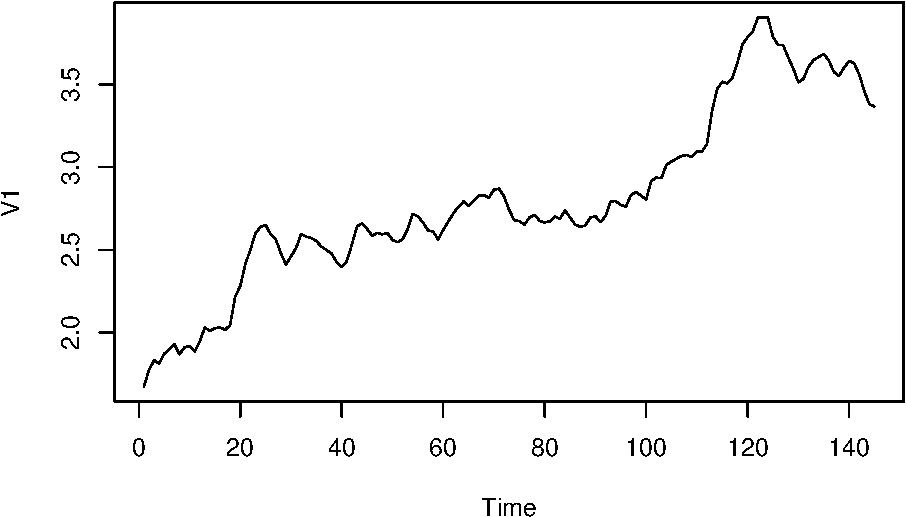
\includegraphics{hw6_files/figure-latex/unnamed-chunk-11-1.pdf}

From the plot, the gas price is non-stationary. A few key observations:

\begin{enumerate}
\item The variance appears constant, so something like a log-transformation
to transform a time series with non-constant variance to a time series with
constant variance seems unnceccessary.
\item The mean appears non-constant.
In particular, the gas prices in the data seem to be trending upwards,
but this is not necessarily the case, e.g., it may be a random walk process.
I think we can summarize the plot with the idea that there is no natural
mean.
\item There are no obvious cycles or seasonality in the data.
\end{enumerate}

We model gas prices as a time series \(\{ Y_t \}\). The \(1\)st order
difference process, \(\{\nabla Y_t\}\), is defined as \[
   \nabla Y_t = Y_t - Y_{t-1}
\] and \(d\)-th order difference process \(\{\nabla^d Y_t\}\) is defined
as \begin{align*}
   \nabla^0 Y_t &= Y_t\\
   \nabla^d Y_t &= \nabla \left(\nabla^{d-1} Y_t\right).
\end{align*} where \(\nabla^0 Y_t\) is the base case in this recursive
definition.

If \(\{Y_t\}\) is non-stationary, it generally has a \(1\)-st or
\(2\)-nd-order difference stationary process. (Higher-order difference
processes are not commonly necessary.)

The first-order difference process of gas prices, \(\{\nabla Y_t\}\),
has the following plots:

\begin{Shaded}
\begin{Highlighting}[]
\NormalTok{Yt.diff }\OtherTok{\textless{}{-}} \FunctionTok{diff}\NormalTok{(Yt,}\DecValTok{1}\NormalTok{)}
\FunctionTok{plot}\NormalTok{(Yt.diff)}
\end{Highlighting}
\end{Shaded}


\includegraphics{hw6_files/figure-latex/unnamed-chunk-12-1.pdf}

\begin{Shaded}
\begin{Highlighting}[]
\FunctionTok{par}\NormalTok{(}\AttributeTok{mfrow=}\FunctionTok{c}\NormalTok{(}\DecValTok{2}\NormalTok{,}\DecValTok{2}\NormalTok{))}
\FunctionTok{hist}\NormalTok{(Yt.diff)}
\FunctionTok{qqnorm}\NormalTok{(Yt.diff)}
\FunctionTok{acf}\NormalTok{(Yt.diff)}
\FunctionTok{pacf}\NormalTok{(Yt.diff)}
\end{Highlighting}
\end{Shaded}

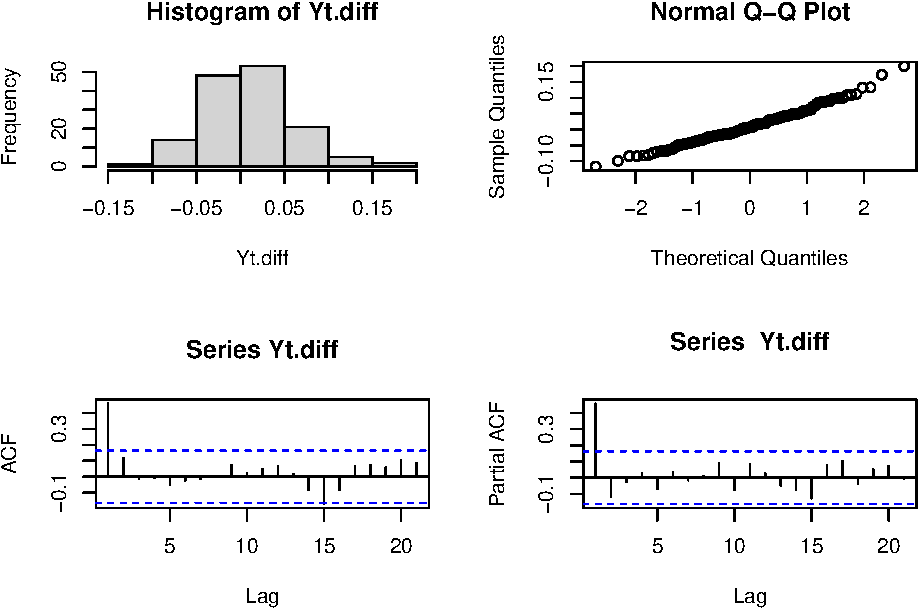
\includegraphics{hw6_files/figure-latex/unnamed-chunk-12-2.pdf}

These plots of \(\{\nabla Y_t\}\) seem to sufficiently approximate white
noise. In subsequent analysis, we will use this differenced time series.

Looking at the ACF, \(\{\nabla Y_t\}\) seems consistent with
\(\operatorname{MA}\), but the PACF is not what we expect. Likewise,
looking at the PACF, \(\{\nabla Y_t\}\) is consistent with
\(\operatorname{AR}\), but the ACF is not what we expect. We have
somewhat of a mixture of both.

We plot the EACF to help decide on plausible ARMA models.

\begin{Shaded}
\begin{Highlighting}[]
\FunctionTok{eacf}\NormalTok{(Yt.diff,}\AttributeTok{ar.max=}\DecValTok{3}\NormalTok{,}\AttributeTok{ma.max=}\DecValTok{3}\NormalTok{)}
\end{Highlighting}
\end{Shaded}

\begin{verbatim}
## AR/MA
##   0 1 2 3
## 0 x o o o
## 1 x o o o
## 2 x x o o
## 3 x o o o
\end{verbatim}

We see that \(\operatorname{ARIMA}(0,1,1)\),
\(\operatorname{ARIMA}(0,1,2)\), and \(\operatorname{ARIMA}(1,1,1)\)
seem like reasonable candidate models for \(\{Y_t\}\).

This does not seem too suprising, given the ACF and PACF plots.

\hypertarget{part-b-1}{%
\subsection{Part (b)}\label{part-b-1}}

\fbox{\begin{minipage}{.8\textwidth}
Perform diagnostic check for each model: check residuals for normality
(histogram, qq-plot), the ACF, and the Ljung-Box test.
\end{minipage}}

We evaluate each of the candidate models in the following subsections.

\hypertarget{model-1-operatornamearma012}{%
\subsubsection{\texorpdfstring{Model 1:
\(\operatorname{ARMA}(0,1,2)\)}{Model 1: \textbackslash operatorname\{ARMA\}(0,1,2)}}\label{model-1-operatornamearma012}}

The histogram, QQ-plot, and ACF of the residuals for
\(\operatorname{ARMA}(0,1,1)\) are given by the following plots.

\begin{Shaded}
\begin{Highlighting}[]
\FunctionTok{library}\NormalTok{(forecast)}
\NormalTok{model1 }\OtherTok{\textless{}{-}} \FunctionTok{Arima}\NormalTok{(Yt,}\AttributeTok{order=}\FunctionTok{c}\NormalTok{(}\DecValTok{0}\NormalTok{,}\DecValTok{1}\NormalTok{,}\DecValTok{2}\NormalTok{))}
\FunctionTok{par}\NormalTok{(}\AttributeTok{mfrow=}\FunctionTok{c}\NormalTok{(}\DecValTok{1}\NormalTok{,}\DecValTok{3}\NormalTok{))}
\FunctionTok{hist}\NormalTok{(model1}\SpecialCharTok{$}\NormalTok{residual,}\AttributeTok{xlab=}\StringTok{"Residual"}\NormalTok{,}\AttributeTok{main=}\StringTok{"ARIMA(0,1,2)"}\NormalTok{)}
\FunctionTok{qqnorm}\NormalTok{(model1}\SpecialCharTok{$}\NormalTok{residual,}\AttributeTok{main=}\StringTok{"QQ{-}plot"}\NormalTok{)}
\FunctionTok{acf}\NormalTok{(model1}\SpecialCharTok{$}\NormalTok{residual,}\AttributeTok{main=}\StringTok{"Residuals"}\NormalTok{)}
\end{Highlighting}
\end{Shaded}

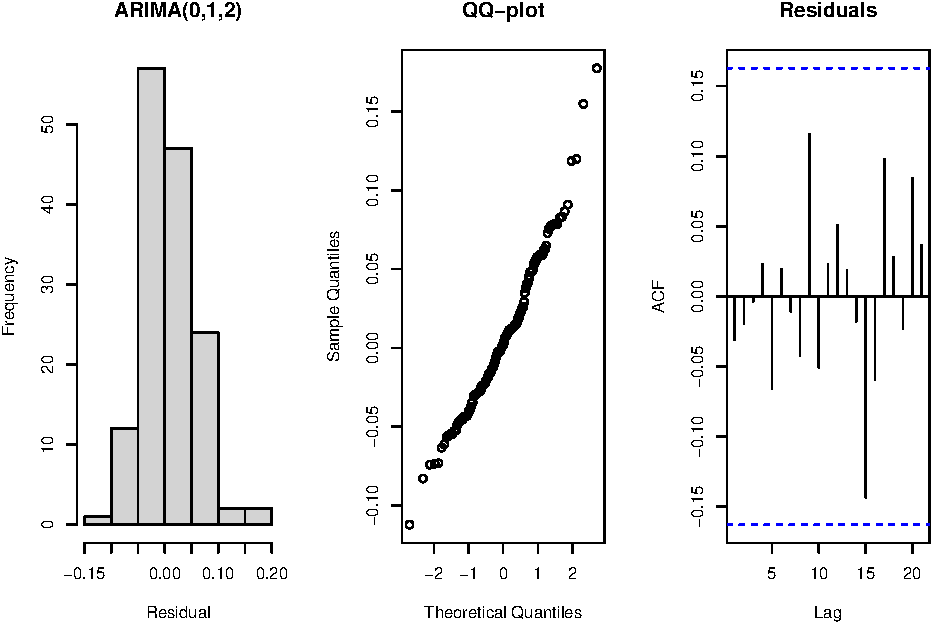
\includegraphics{hw6_files/figure-latex/unnamed-chunk-14-1.pdf}

The residuals seem like a reasonable approximation of white noise. Next,
we do a Box-Ljung test:

\begin{Shaded}
\begin{Highlighting}[]
\NormalTok{K }\OtherTok{\textless{}{-}} \DecValTok{30}
\NormalTok{p }\OtherTok{\textless{}{-}} \DecValTok{0}
\NormalTok{q }\OtherTok{\textless{}{-}} \DecValTok{2}
\FunctionTok{Box.test}\NormalTok{(model1}\SpecialCharTok{$}\NormalTok{residuals,}
         \AttributeTok{lag=}\NormalTok{K,}
         \AttributeTok{type=}\StringTok{"Ljung{-}Box"}\NormalTok{,}
         \AttributeTok{fitdf=}\NormalTok{p}\SpecialCharTok{+}\NormalTok{q)}
\end{Highlighting}
\end{Shaded}

\begin{verbatim}
## 
##  Box-Ljung test
## 
## data:  model1$residuals
## X-squared = 17.798, df = 28, p-value = 0.9311
\end{verbatim}

The observed test statistic is compatible with the hypothesis that the
residuals are white noise.

\hypertarget{model-2-operatornamearma011}{%
\subsubsection{\texorpdfstring{Model 2:
\(\operatorname{ARMA}(0,1,1)\)}{Model 2: \textbackslash operatorname\{ARMA\}(0,1,1)}}\label{model-2-operatornamearma011}}

The histogram, QQ-plot, and ACF of the residuals for
\(\operatorname{ARMA}(0,1,1)\) are given by the following plots.

\begin{Shaded}
\begin{Highlighting}[]
\FunctionTok{library}\NormalTok{(forecast)}
\NormalTok{model2 }\OtherTok{\textless{}{-}} \FunctionTok{Arima}\NormalTok{(Yt,}\AttributeTok{order=}\FunctionTok{c}\NormalTok{(}\DecValTok{0}\NormalTok{,}\DecValTok{1}\NormalTok{,}\DecValTok{1}\NormalTok{))}
\FunctionTok{par}\NormalTok{(}\AttributeTok{mfrow=}\FunctionTok{c}\NormalTok{(}\DecValTok{1}\NormalTok{,}\DecValTok{3}\NormalTok{))}
\FunctionTok{hist}\NormalTok{(model2}\SpecialCharTok{$}\NormalTok{residual,}\AttributeTok{xlab=}\StringTok{"Residual"}\NormalTok{,}\AttributeTok{main=}\StringTok{"ARIMA(0,1,1)"}\NormalTok{)}
\FunctionTok{qqnorm}\NormalTok{(model2}\SpecialCharTok{$}\NormalTok{residual,}\AttributeTok{main=}\StringTok{"QQ{-}plot"}\NormalTok{)}
\FunctionTok{acf}\NormalTok{(model2}\SpecialCharTok{$}\NormalTok{residual,}\AttributeTok{main=}\StringTok{"Residuals"}\NormalTok{)}
\end{Highlighting}
\end{Shaded}


\includegraphics{hw6_files/figure-latex/unnamed-chunk-16-1.pdf}

The residuals seem like a reasonable approximation of white noise. Next,
we do a Box-Ljung test:

\begin{Shaded}
\begin{Highlighting}[]
\NormalTok{p }\OtherTok{\textless{}{-}} \DecValTok{0}
\NormalTok{q }\OtherTok{\textless{}{-}} \DecValTok{1}
\FunctionTok{Box.test}\NormalTok{(model2}\SpecialCharTok{$}\NormalTok{residuals,}
         \AttributeTok{lag=}\NormalTok{K,}
         \AttributeTok{type=}\StringTok{"Ljung{-}Box"}\NormalTok{,}
         \AttributeTok{fitdf=}\NormalTok{p}\SpecialCharTok{+}\NormalTok{q)}
\end{Highlighting}
\end{Shaded}

\begin{verbatim}
## 
##  Box-Ljung test
## 
## data:  model2$residuals
## X-squared = 22.266, df = 29, p-value = 0.809
\end{verbatim}

The observed test statistic is compatible with the hypothesis that the
residuals are white noise.

\hypertarget{model-3-operatornamearma111}{%
\subsubsection{\texorpdfstring{Model 3:
\(\operatorname{ARMA}(1,1,1)\)}{Model 3: \textbackslash operatorname\{ARMA\}(1,1,1)}}\label{model-3-operatornamearma111}}

The histogram, QQ-plot, and ACF of the residuals for
\(\operatorname{ARMA}(1,1,1)\) are given by the following plots.

\begin{Shaded}
\begin{Highlighting}[]
\FunctionTok{library}\NormalTok{(forecast)}
\NormalTok{model3 }\OtherTok{\textless{}{-}} \FunctionTok{Arima}\NormalTok{(Yt,}\AttributeTok{order=}\FunctionTok{c}\NormalTok{(}\DecValTok{1}\NormalTok{,}\DecValTok{1}\NormalTok{,}\DecValTok{1}\NormalTok{))}
\FunctionTok{par}\NormalTok{(}\AttributeTok{mfrow=}\FunctionTok{c}\NormalTok{(}\DecValTok{1}\NormalTok{,}\DecValTok{3}\NormalTok{))}
\FunctionTok{hist}\NormalTok{(model3}\SpecialCharTok{$}\NormalTok{residual,}\AttributeTok{xlab=}\StringTok{"Residual"}\NormalTok{,}\AttributeTok{main=}\StringTok{"ARIMA(1,1,1)"}\NormalTok{)}
\FunctionTok{qqnorm}\NormalTok{(model3}\SpecialCharTok{$}\NormalTok{residual,}\AttributeTok{main=}\StringTok{"QQ{-}plot"}\NormalTok{)}
\FunctionTok{acf}\NormalTok{(model3}\SpecialCharTok{$}\NormalTok{residual,}\AttributeTok{main=}\StringTok{"Residuals"}\NormalTok{)}
\end{Highlighting}
\end{Shaded}

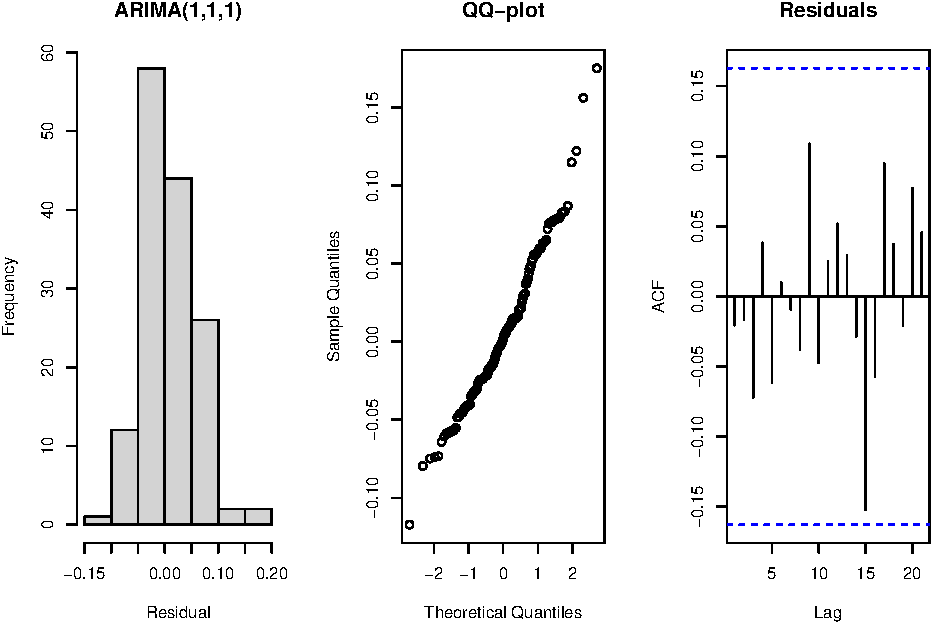
\includegraphics{hw6_files/figure-latex/unnamed-chunk-18-1.pdf}

The residuals seem like a reasonable approximation of white noise. Next,
we do a Box-Ljung test:

\begin{Shaded}
\begin{Highlighting}[]
\NormalTok{p }\OtherTok{\textless{}{-}} \DecValTok{1}
\NormalTok{q }\OtherTok{\textless{}{-}} \DecValTok{1}
\FunctionTok{Box.test}\NormalTok{(model3}\SpecialCharTok{$}\NormalTok{residuals,}
         \AttributeTok{lag=}\NormalTok{K,}
         \AttributeTok{type=}\StringTok{"Ljung{-}Box"}\NormalTok{,}
         \AttributeTok{fitdf=}\NormalTok{p}\SpecialCharTok{+}\NormalTok{q)}
\end{Highlighting}
\end{Shaded}

\begin{verbatim}
## 
##  Box-Ljung test
## 
## data:  model3$residuals
## X-squared = 18.654, df = 28, p-value = 0.9085
\end{verbatim}

The observed test statistic is compatible with the hypothesis that the
residuals are white noise.

\hypertarget{part-c-1}{%
\subsection{Part (c)}\label{part-c-1}}

\fbox{\begin{minipage}{.8\textwidth}
Choose a final model (if all fit fine, choose the one with the smallest AIC).
Report your final model and calculate forecasts and prediction intervals for 5
future values.
Display the forecasts and prediction bands visually like.
\end{minipage}}

Both models fit fine, so we will use the model with the minimum AIC.

\begin{Shaded}
\begin{Highlighting}[]
\FunctionTok{round}\NormalTok{(}\FunctionTok{c}\NormalTok{(model1}\SpecialCharTok{$}\NormalTok{aic,model2}\SpecialCharTok{$}\NormalTok{aic,model3}\SpecialCharTok{$}\NormalTok{aic),}\DecValTok{3}\NormalTok{)}
\end{Highlighting}
\end{Shaded}

\begin{verbatim}
## [1] -459.062 -455.297 -458.351
\end{verbatim}

We see that the \(\operatorname{ARIMA}(0,1,2)\) model for \(\{Y_t\}\)
has the minimum AIC of these models with an AIC of -459.062, so we
choose this model.

The model summary is given by:

\begin{Shaded}
\begin{Highlighting}[]
\FunctionTok{summary}\NormalTok{(model1)}
\end{Highlighting}
\end{Shaded}

\begin{verbatim}
## Series: Yt 
## ARIMA(0,1,2) 
## 
## Coefficients:
##          ma1     ma2
##       0.5433  0.1946
## s.e.  0.0843  0.0779
## 
## sigma^2 = 0.002345:  log likelihood = 232.53
## AIC=-459.06   AICc=-458.89   BIC=-450.15
## 
## Training set error measures:
##                       ME       RMSE        MAE       MPE     MAPE      MASE
## Training set 0.006717107 0.04791789 0.03709482 0.2712316 1.381354 0.8635071
##                     ACF1
## Training set -0.03092411
\end{verbatim}

The forecast and prediction intervals for the
\(\operatorname{ARMA}(1,1,1)\) model are given by:

\begin{Shaded}
\begin{Highlighting}[]
\FunctionTok{library}\NormalTok{(forecast)}
\NormalTok{model1.fc }\OtherTok{\textless{}{-}} \FunctionTok{forecast}\NormalTok{(Yt[}\DecValTok{125}\SpecialCharTok{:}\DecValTok{145}\NormalTok{],}\AttributeTok{model=}\NormalTok{model1,}\AttributeTok{h=}\DecValTok{5}\NormalTok{)}
\FunctionTok{plot}\NormalTok{(model1.fc)}
\end{Highlighting}
\end{Shaded}


\includegraphics{hw6_files/figure-latex/unnamed-chunk-22-1.pdf}

\hypertarget{additional-thoughts-evaluating-model-performance-via-data-splitting}{%
\subsection{Additional thoughts: evaluating model performance via data
splitting}\label{additional-thoughts-evaluating-model-performance-via-data-splitting}}

Out of curiosity, we evaluate the performance of the selected model, the
fitted \(\operatorname{ARIMIA}(1,1,1)\) model, via data splitting, i.e.,
learning on a training set and comparing the forecast with the test set.

\begin{Shaded}
\begin{Highlighting}[]
\FunctionTok{library}\NormalTok{(forecast)}

\NormalTok{Yt.train }\OtherTok{\textless{}{-}} \FunctionTok{ts}\NormalTok{(Yt[}\DecValTok{1}\SpecialCharTok{:}\DecValTok{115}\NormalTok{],}\AttributeTok{start=}\DecValTok{1}\NormalTok{)}
\NormalTok{Yt.test }\OtherTok{\textless{}{-}} \FunctionTok{ts}\NormalTok{(Yt[}\DecValTok{116}\SpecialCharTok{:}\DecValTok{145}\NormalTok{],}\AttributeTok{start=}\DecValTok{116}\NormalTok{)}

\NormalTok{model1.train }\OtherTok{\textless{}{-}} \FunctionTok{Arima}\NormalTok{(Yt.train,}\AttributeTok{order=}\FunctionTok{c}\NormalTok{(}\DecValTok{0}\NormalTok{,}\DecValTok{1}\NormalTok{,}\DecValTok{2}\NormalTok{))}
\NormalTok{model1.train.fc }\OtherTok{\textless{}{-}} \FunctionTok{forecast}\NormalTok{(Yt.train,}\AttributeTok{model=}\NormalTok{model1.train,}\AttributeTok{h=}\DecValTok{30}\NormalTok{)}

\FunctionTok{plot}\NormalTok{(model1.train.fc)}
\FunctionTok{lines}\NormalTok{(Yt.test, }\AttributeTok{lty=}\DecValTok{2}\NormalTok{)}
\end{Highlighting}
\end{Shaded}


\includegraphics{hw6_files/figure-latex/unnamed-chunk-23-1.pdf}

Over the long run, the forecast is not bad, but it is not very sensitive
to recent history (the positive trend near the end of the training time
series). Out of curiosity, we fit a double exponential smoothing model
to the training set and then plot its forecast and prediction intervals:

\begin{Shaded}
\begin{Highlighting}[]
\NormalTok{dema.train }\OtherTok{\textless{}{-}} \FunctionTok{holt}\NormalTok{(Yt.train,}\AttributeTok{h=}\DecValTok{30}\NormalTok{,}\AttributeTok{initial=}\StringTok{"optimal"}\NormalTok{)}
\NormalTok{dema.train.fc }\OtherTok{\textless{}{-}} \FunctionTok{forecast}\NormalTok{(Yt.train,}\AttributeTok{model=}\NormalTok{dema.train,}\AttributeTok{h=}\DecValTok{30}\NormalTok{)}
\FunctionTok{plot}\NormalTok{(dema.train.fc)}
\FunctionTok{lines}\NormalTok{(Yt.test,}\AttributeTok{lty=}\DecValTok{2}\NormalTok{)}
\end{Highlighting}
\end{Shaded}

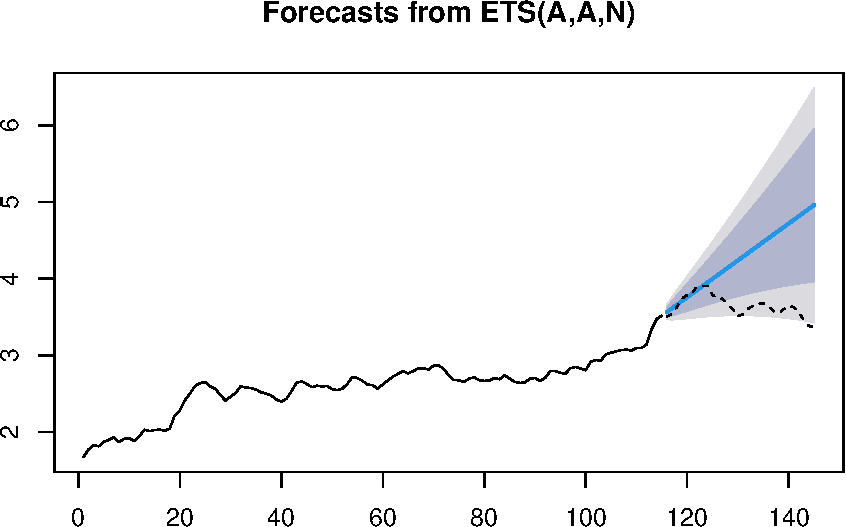
\includegraphics{hw6_files/figure-latex/unnamed-chunk-24-1.pdf}

This produces a better short-term forecast that follows the recent trend
found at the end of the training time series. As the forecast extends
further into the future, it diverges significantly from the test data.
(Forecasts will often perform better if any trends are dampened over
time, asymptotically converging to a \(0\) slope. Such a dampening
effect would improve the forecast for this model.)

As a famous quote puts, ``It is difficult to make predictions,
especially about the future.'' Due to the often extreme uncertainty
about the future, we tend not to put much stock in long term forecasting
(unless the data is highly regular, e.g., we assume the Sun will
continue to rise in the morning long into the future). Given this
uncertainty and the \emph{present bias} (we tend to discount far-off
rewards), we usually seek a model that we expect to perform well on
near-term forecasts. On this metric, we are inclined to prefer the
double exponential smoothing model presented above.

\hypertarget{problem-3}{%
\section{Problem 3}\label{problem-3}}

A data set of public transportation boardings in Denver from August 2000
through December 2005 are in the boardings object in the TSA package.
These data are already logged.

\begin{Shaded}
\begin{Highlighting}[]
\FunctionTok{library}\NormalTok{(TSA)}
\FunctionTok{data}\NormalTok{(boardings)}
\NormalTok{log.boardings }\OtherTok{=}\NormalTok{ boardings[,}\DecValTok{1}\NormalTok{]}
\FunctionTok{print}\NormalTok{(log.boardings)}
\end{Highlighting}
\end{Shaded}

\begin{verbatim}
##           Jan      Feb      Mar      Apr      May      Jun      Jul      Aug
## 2000                                                                12.49114
## 2001 12.45759 12.51886 12.49804 12.52874 12.52780 12.52162 12.48012 12.52364
## 2002 12.50106 12.52229 12.49063 12.55226 12.54457 12.51336 12.46190 12.51414
## 2003 12.49483 12.53297 12.44026 12.50992 12.50498 12.44860 12.44798 12.48586
## 2004 12.47789 12.54076 12.54592 12.56986 12.57247 12.49189 12.47962 12.51481
## 2005 12.53937 12.58296 12.57383 12.59280 12.58038 12.52468 12.51634 12.57870
## 2006 12.60070 12.62888 12.61389                                             
##           Sep      Oct      Nov      Dec
## 2000 12.58577 12.53457 12.52406 12.39809
## 2001 12.60110 12.58120 12.54482 12.46953
## 2002 12.56313 12.55305 12.54575 12.46286
## 2003 12.58046 12.55216 12.50488 12.42697
## 2004 12.62301 12.59301 12.56187 12.45818
## 2005 12.69752 12.66482 12.63930 12.52714
## 2006
\end{verbatim}

\hypertarget{part-a-2}{%
\subsection{Part (a)}\label{part-a-2}}

\fbox{\begin{minipage}{.8\textwidth}
Give a time series plot of these data.
Comment on the plot and any seasonality.
Is it reasonable to use a stationary model for this time series?
\end{minipage}}

The time series is plotted with:

\begin{Shaded}
\begin{Highlighting}[]
\FunctionTok{plot}\NormalTok{(log.boardings)}
\end{Highlighting}
\end{Shaded}

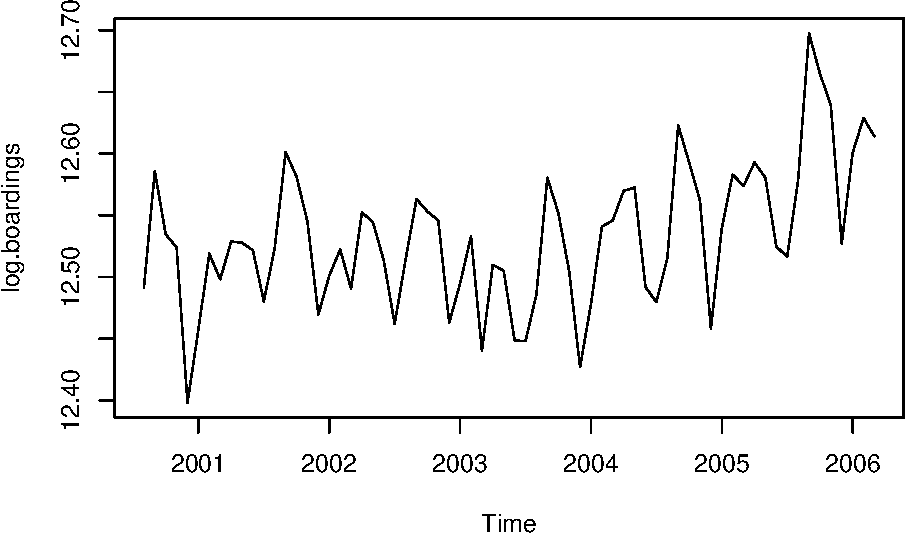
\includegraphics{hw6_files/figure-latex/unnamed-chunk-26-1.pdf}

First, there does appear to be a slight seasonable component, although
admittedly it is not especially pronounced.

It does not appear to be stationary. We perform the Dickey-Fuller test
to further convince ourselves:

\begin{Shaded}
\begin{Highlighting}[]
\NormalTok{tseries}\SpecialCharTok{::}\FunctionTok{adf.test}\NormalTok{(log.boardings)}
\end{Highlighting}
\end{Shaded}

\begin{verbatim}
## 
##  Augmented Dickey-Fuller Test
## 
## data:  log.boardings
## Dickey-Fuller = -2.163, Lag order = 4, p-value = 0.5089
## alternative hypothesis: stationary
\end{verbatim}

At this \(p\)-value, we do not reject the null hypothesis of
non-stationary data. We take the difference and perform the
Dickey-Fuller test on that transformation:

\begin{Shaded}
\begin{Highlighting}[]
\NormalTok{log.boardings.diff }\OtherTok{\textless{}{-}} \FunctionTok{diff}\NormalTok{(log.boardings,}\DecValTok{1}\NormalTok{)}
\FunctionTok{plot}\NormalTok{(log.boardings.diff)}
\end{Highlighting}
\end{Shaded}


\includegraphics{hw6_files/figure-latex/unnamed-chunk-28-1.pdf}

\begin{Shaded}
\begin{Highlighting}[]
\NormalTok{tseries}\SpecialCharTok{::}\FunctionTok{adf.test}\NormalTok{(log.boardings.diff)}
\end{Highlighting}
\end{Shaded}

\begin{verbatim}
## 
##  Augmented Dickey-Fuller Test
## 
## data:  log.boardings.diff
## Dickey-Fuller = -6.939, Lag order = 4, p-value = 0.01
## alternative hypothesis: stationary
\end{verbatim}

The plot seems to resemble a stationary process. Moreover, the
\(p\)-value of the Dickey-Fuller hypothesis test is around \(0.01\),
which we consider to be very strong evidence against the null hypothesis
of non-stationary data.

\hypertarget{part-b-2}{%
\subsection{Part (b)}\label{part-b-2}}

\fbox{Plot the sample ACF of the series. Interpret what the plot tells you.}

We plot the ACF with:

\begin{Shaded}
\begin{Highlighting}[]
\FunctionTok{par}\NormalTok{(}\AttributeTok{mfrow=}\FunctionTok{c}\NormalTok{(}\DecValTok{1}\NormalTok{,}\DecValTok{2}\NormalTok{))}
\FunctionTok{acf}\NormalTok{(log.boardings.diff)}
\FunctionTok{pacf}\NormalTok{(log.boardings.diff)}
\end{Highlighting}
\end{Shaded}

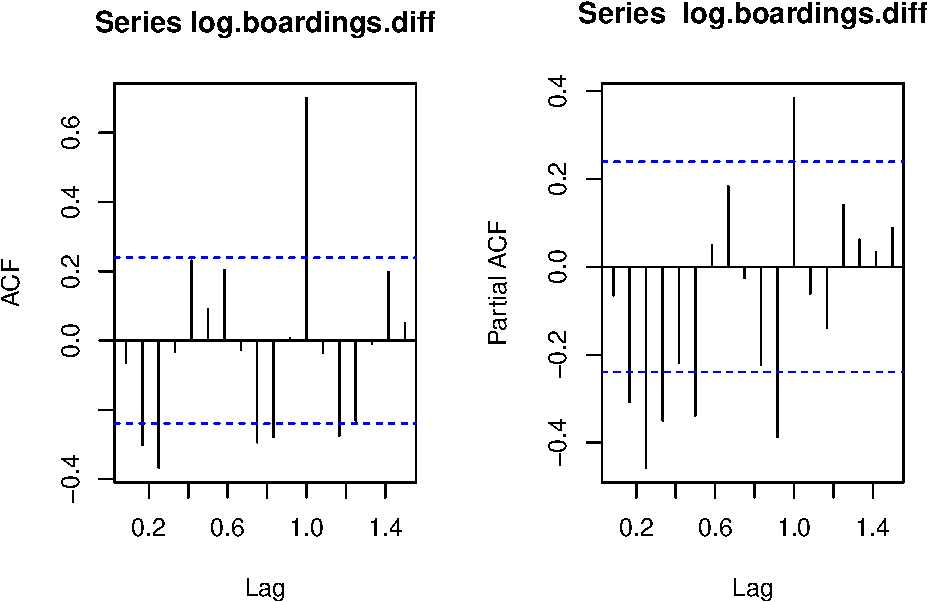
\includegraphics{hw6_files/figure-latex/unnamed-chunk-29-1.pdf}

This ACF diverges from the theoretical ACF of stationary data, but a
\(2\)-nd order difference does not improve the situation. This does not
seem too bad.

\hypertarget{part-c-2}{%
\subsection{Part (c)}\label{part-c-2}}

\fbox{\begin{minipage}{.8\textwidth}
Choose a seasonal ARIMA model that fits the data.
Write down your model and the corresponding AIC.
\end{minipage}}

We look at the EACF with:

\begin{Shaded}
\begin{Highlighting}[]
\FunctionTok{library}\NormalTok{(TSA)}
\FunctionTok{eacf}\NormalTok{(log.boardings.diff,}\AttributeTok{ar.max=}\DecValTok{4}\NormalTok{,}\AttributeTok{ma.max=}\DecValTok{4}\NormalTok{)}
\end{Highlighting}
\end{Shaded}

\begin{verbatim}
## AR/MA
##   0 1 2 3 4
## 0 o x x o o
## 1 o o x o o
## 2 x x o o o
## 3 x o o o o
## 4 x x o o o
\end{verbatim}

This EACF indicates \(\operatorname{ARIMA}(p,d=1,q)\) with
\((p,q) \in \{(0,0),(1,0),(1,1)\}\).

Given the seasonality of the data, we elect to fit a seasonal ARIMA
model with parameters \((p,d,q) \times (P,D,Q)\), found by using the
\emph{auto-arima} function and the data indicates a periodicity of
\(s=12\) (\(S_t = S_{t+s}\)).

\begin{Shaded}
\begin{Highlighting}[]
\NormalTok{fit }\OtherTok{\textless{}{-}} \FunctionTok{auto.arima}\NormalTok{(log.boardings)}
\FunctionTok{summary}\NormalTok{(fit)}
\end{Highlighting}
\end{Shaded}

\begin{verbatim}
## Series: log.boardings 
## ARIMA(1,1,0)(0,1,1)[12] 
## 
## Coefficients:
##           ar1     sma1
##       -0.2919  -0.6089
## s.e.   0.1281   0.2280
## 
## sigma^2 = 0.0005886:  log likelihood = 126.56
## AIC=-247.12   AICc=-246.65   BIC=-241.1
## 
## Training set error measures:
##                        ME       RMSE       MAE         MPE      MAPE      MASE
## Training set 0.0002045332 0.02141851 0.0154136 0.001459963 0.1230202 0.4291575
##                    ACF1
## Training set 0.04400124
\end{verbatim}

\begin{Shaded}
\begin{Highlighting}[]
\FunctionTok{print}\NormalTok{(fit}\SpecialCharTok{$}\NormalTok{aic)}
\end{Highlighting}
\end{Shaded}

\begin{verbatim}
## [1] -247.1219
\end{verbatim}

We see that the AIC is \(-247.1219\) and the best fit model is of type
\[
   \operatorname{Seasonal-ARIMA}(p=1,d=1,q=0) \times (P=0,D=1,Q=1).
\] with coefficients given by

\begin{Shaded}
\begin{Highlighting}[]
\FunctionTok{coef}\NormalTok{(fit)}
\end{Highlighting}
\end{Shaded}

\begin{verbatim}
##        ar1       sma1 
## -0.2918525 -0.6088785
\end{verbatim}

\hypertarget{part-d-1}{%
\subsection{Part (d)}\label{part-d-1}}

\fbox{\begin{minipage}{.8\textwidth}
Check residuals for normality (histogram, qq-plot), for independence (ACF and
the Ljung-Box test).
Comment on your findings.
\end{minipage}}

We plot a histogram, Q-Q plot, and ACF of the residuals with:

\begin{Shaded}
\begin{Highlighting}[]
\FunctionTok{par}\NormalTok{(}\AttributeTok{mfrow=}\FunctionTok{c}\NormalTok{(}\DecValTok{1}\NormalTok{,}\DecValTok{3}\NormalTok{))}
\FunctionTok{hist}\NormalTok{(fit}\SpecialCharTok{$}\NormalTok{residual,}\AttributeTok{xlab=}\StringTok{"Residual"}\NormalTok{,}\AttributeTok{main=}\StringTok{"Seasonal ARIMA"}\NormalTok{)}
\FunctionTok{qqnorm}\NormalTok{(fit}\SpecialCharTok{$}\NormalTok{residual,}\AttributeTok{main=}\StringTok{"QQ{-}plot of residuals"}\NormalTok{)}
\FunctionTok{acf}\NormalTok{(fit}\SpecialCharTok{$}\NormalTok{residual,}\AttributeTok{main=}\StringTok{"ACF of residuals"}\NormalTok{)}
\end{Highlighting}
\end{Shaded}

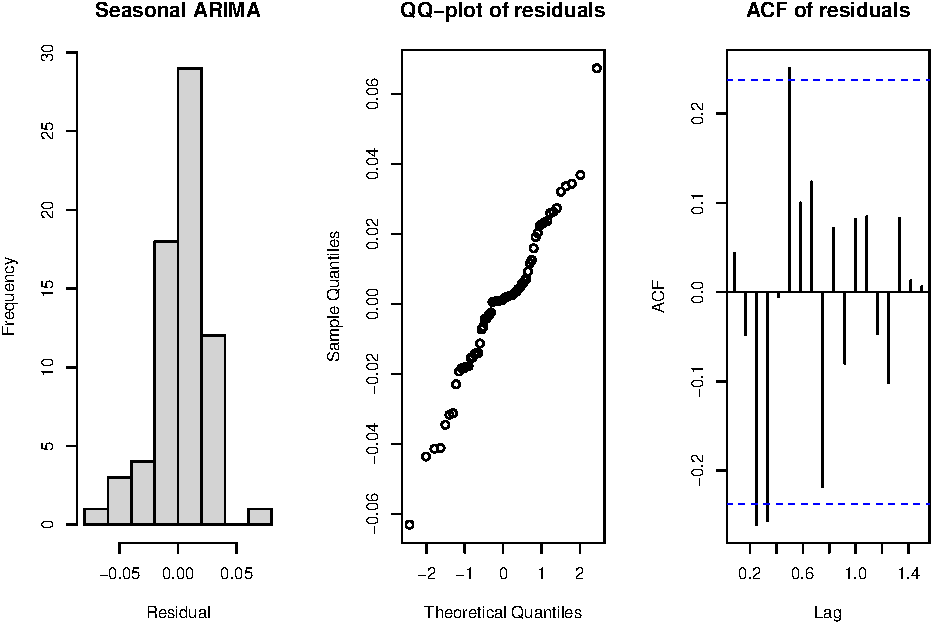
\includegraphics{hw6_files/figure-latex/unnamed-chunk-33-1.pdf}

We are not entirely comfortable with these plots representing idealized
white noise, but real data sets are not typically going to have a data
generating process that is truly distributed according to the ARIMA
models, so some discrepencies are expected.

As the saying goes, all models are wrong, but hopefully some are useful.
These plots satisfy us that we have sufficiently modeled the significant
patterns in the data.

However, we conduct one last hypothesis test on the residuals with:

\begin{Shaded}
\begin{Highlighting}[]
\FunctionTok{Box.test}\NormalTok{(fit}\SpecialCharTok{$}\NormalTok{residuals,}
         \AttributeTok{lag=}\NormalTok{K,}
         \AttributeTok{type=}\StringTok{"Ljung{-}Box"}\NormalTok{,}
         \AttributeTok{fitdf=}\DecValTok{3}\NormalTok{)}
\end{Highlighting}
\end{Shaded}

\begin{verbatim}
## 
##  Box-Ljung test
## 
## data:  fit$residuals
## X-squared = 38.809, df = 27, p-value = 0.06594
\end{verbatim}

According to the Box-Ljung test, at a typical significance level
\(\alpha=0.05\), the residuals are compatible with a white noise
process.

\hypertarget{additional-plots}{%
\subsubsection{Additional plots}\label{additional-plots}}

For fun, we do some forecasting with the model:

\begin{Shaded}
\begin{Highlighting}[]
\FunctionTok{library}\NormalTok{(forecast)}

\FunctionTok{plot}\NormalTok{(log.boardings,}\AttributeTok{lty=}\DecValTok{2}\NormalTok{)}
\FunctionTok{lines}\NormalTok{(fit}\SpecialCharTok{$}\NormalTok{fitted,}\AttributeTok{col=}\StringTok{"green"}\NormalTok{)}
\end{Highlighting}
\end{Shaded}

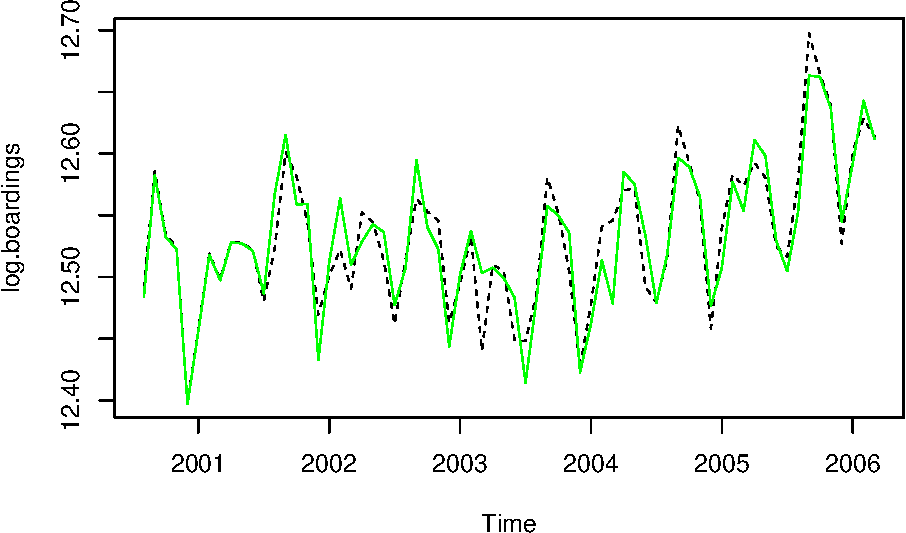
\includegraphics{hw6_files/figure-latex/unnamed-chunk-35-1.pdf}

\begin{Shaded}
\begin{Highlighting}[]
\NormalTok{fit.fc }\OtherTok{\textless{}{-}} \FunctionTok{forecast}\NormalTok{(log.boardings,}\AttributeTok{model=}\NormalTok{fit,}\AttributeTok{h=}\DecValTok{100}\NormalTok{)}
\FunctionTok{plot}\NormalTok{(fit.fc)}
\end{Highlighting}
\end{Shaded}

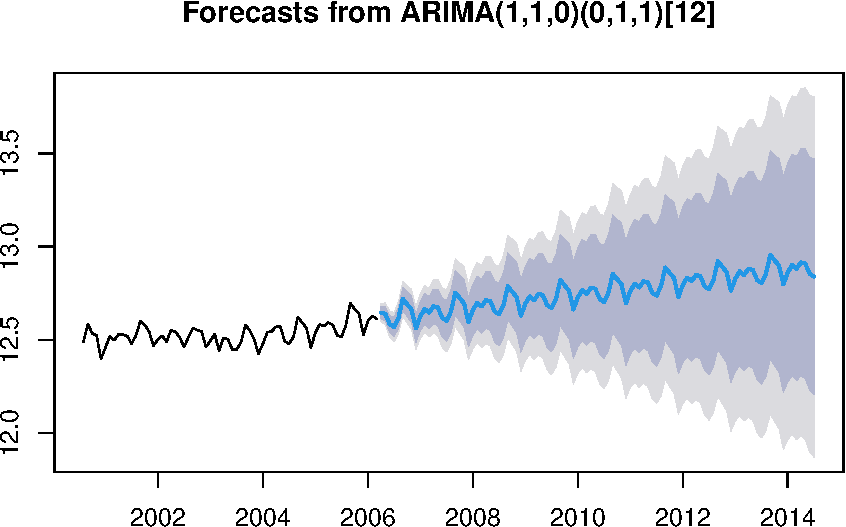
\includegraphics{hw6_files/figure-latex/unnamed-chunk-35-2.pdf} Note
that this is with the log-transformed time series, so the forecast of
the original time series is given by taking the exponential value of
these forecasts.

\end{document}
